\begin{tikzpicture}
\node[anchor=south west,inner sep=0] at (0,0) {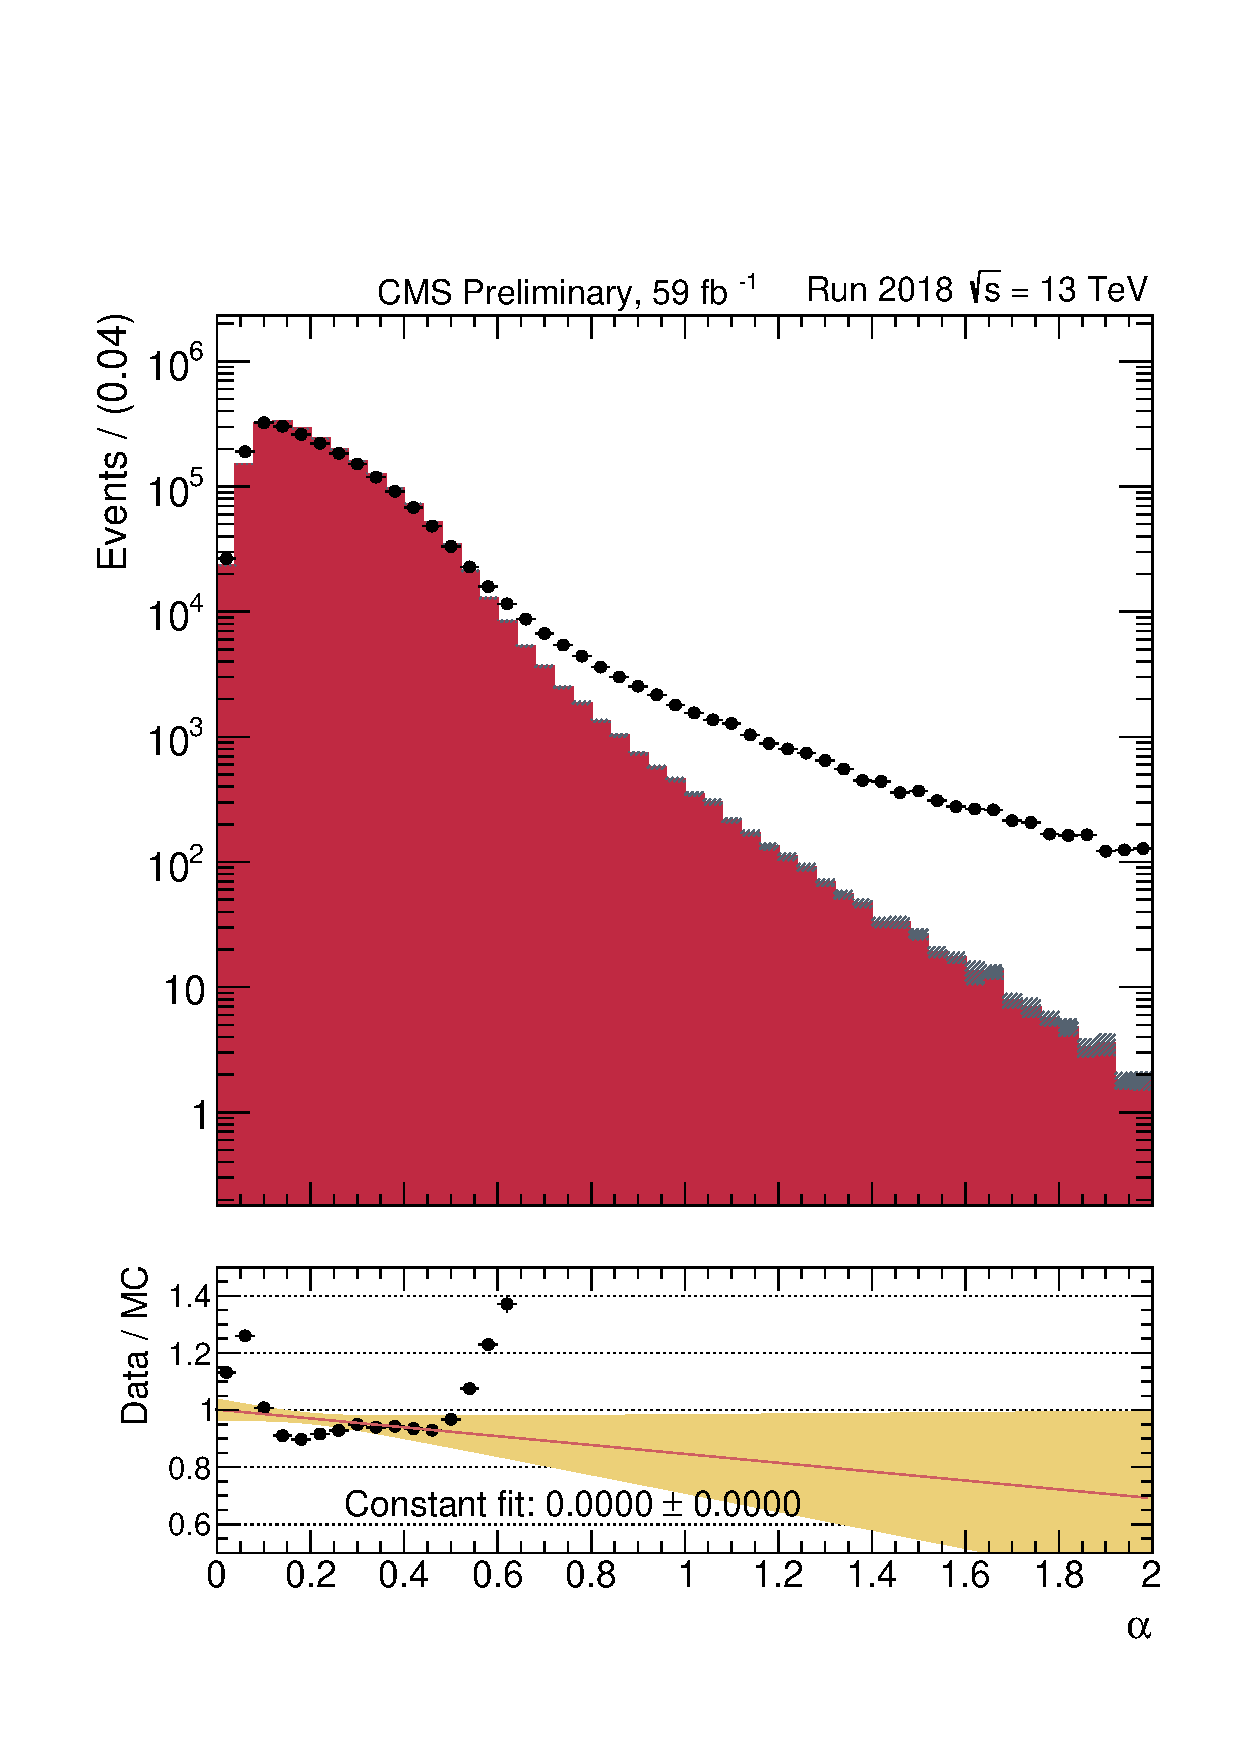
\includegraphics[width=8cm]{\PhDthesisdir/contents/chapter-JERC/plots/my_plots/distributions/2018/source/alpha_log.pdf}};

% above txt
\fill [white] (1.2, 7.31) rectangle (7.6,7.7);
\draw (7.6, 7.5) node [left] {\footnotesize Run 2018 ABCD, \SI{59}{\femto\barn^{-1}} (\SI{13}{\TeV})};

% masks
\fill [white] (1, 0) rectangle (8,.55);
\fill [white] (0, 0) rectangle (.9,7.5);

% X axis
\foreach \val in {10, 20, ..., 70}{
\draw ({1.475+(7.53-1.475)*(\val-10)/(70-10)}, .45) node {\small \val};
}
\draw (7.5, .15) node [left] {\normalsize Nombre d'interactions d'empilement};

% Y axis
\foreach \pos/\val in {0/10^{-5}, 1/10^{-4}, 2/10^{-3}, 3/10^{-2}, 4/10^{-1}, 5/1}{
\draw (1.075, {.6+\pos/5*(7.3-.6)}) node [left] {\small $\val$};
}
\draw (.25, 7.25) node [left, rotate=90] {\normalsize Probabilité};

	\def\xmin{0} \def\xmax{8} \def\ymin{0} \def\ymax{10}
	% Grilles
	\draw [step=0.1cm,lightgray,ultra thin]  (\xmin,\ymin) grid (\xmax,\ymax);
	\draw [step=0.5cm,lightgray, thin] (\xmin,\ymin) grid (\xmax,\ymax);
	\draw [step=1cm,lightgray, thick] (\xmin,\ymin) grid (\xmax,\ymax);
	\draw [step=5cm,lightgray,very thick] (\xmin,\ymin) grid (\xmax,\ymax);
	

\end{tikzpicture}
